\documentclass[serif,mathserif,final]{beamer}
\mode<presentation>{\usetheme{Lankton}}
\usepackage{amsmath,amsfonts,amssymb,pxfonts,eulervm,xspace}
\usepackage{graphicx, ragged2e}
\graphicspath{{./figures/}}
\usepackage[orientation=landscape,size=a0,scale=1.6,debug]{beamerposter}

%-- Header and footer information ----------------------------------
\newcommand{\footleft}{This work performed under the auspices of the U.S. Department of Energy by Lawrence Livermore National Laboratory under Contract DE-AC52-07NA27344.}
\newcommand{\footright}{IM Review and Release \#\hspace{15ex}}
\title{Slacking-conscious Lightweight Loop Scheduling for Improving Scalability of Bulk-synchronous MPI applications}
\author{Vivek Kale$^1$$^2$ \quad Todd Gamblin$^2$ \quad Torsten Hoefler$^1$ 
\quad Bronis R. de Supinski$^2$ \quad William D. Gropp$^1$}
\institute{$^1$Department of Computer Science, University of Illinois at Urbana-Champaign 
\quad $^2$Lawrence Livermore National Laboratory}
%------------------------------------------------------------------- 

%-- Main Document --------------------------------------------------
\begin{document}
\begin{frame}{}
  \begin{columns}[t]
    %-- Column 1 ---------------------------------------------------
    \begin{column}{0.28\linewidth} 
      %-- Block 1-1
      \begin{block}{    }
      \end{block}

      \vspace{1.5ex}

      %-- Block 1-2
      \begin{block}{    }
         
         \vspace{2ex}

         \begin{figure}[htb]
         \centering
         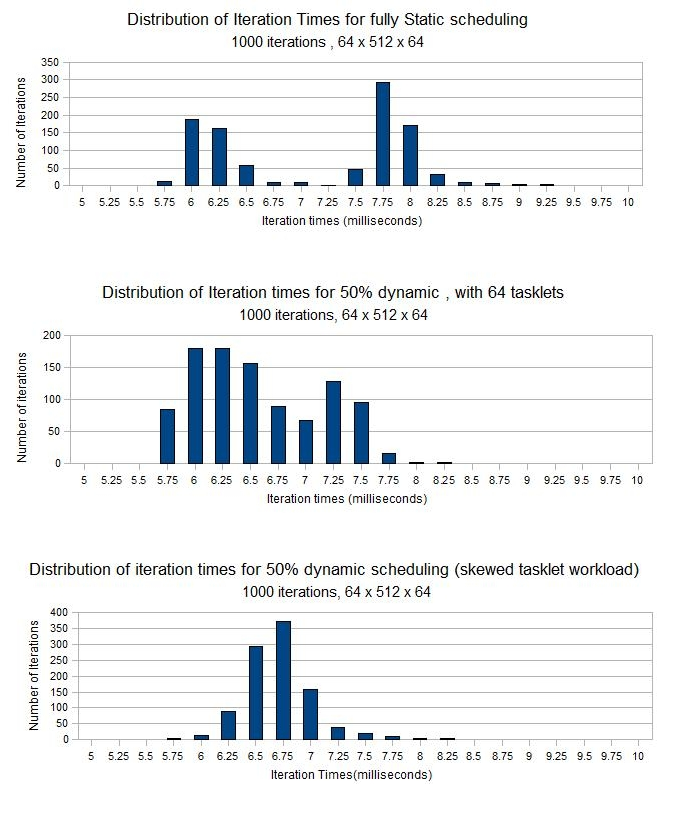
\includegraphics[width=.4\columnwidth]{images/IterationTimingsHisto.png}
         \caption{Iteration Timing Histogram indicating performance variations across multiple runs. }
         \end{figure}
         \vspace{3ex}
         {\footnotesize}
      \end{block}
    \end{column}%1


    %-- Column 2 ---------------------------------------------------
    \begin{column}{0.4\linewidth}

      %-- Block 2-1
      \begin{block}{}

       \begin{figure}[htb]
          \centering
          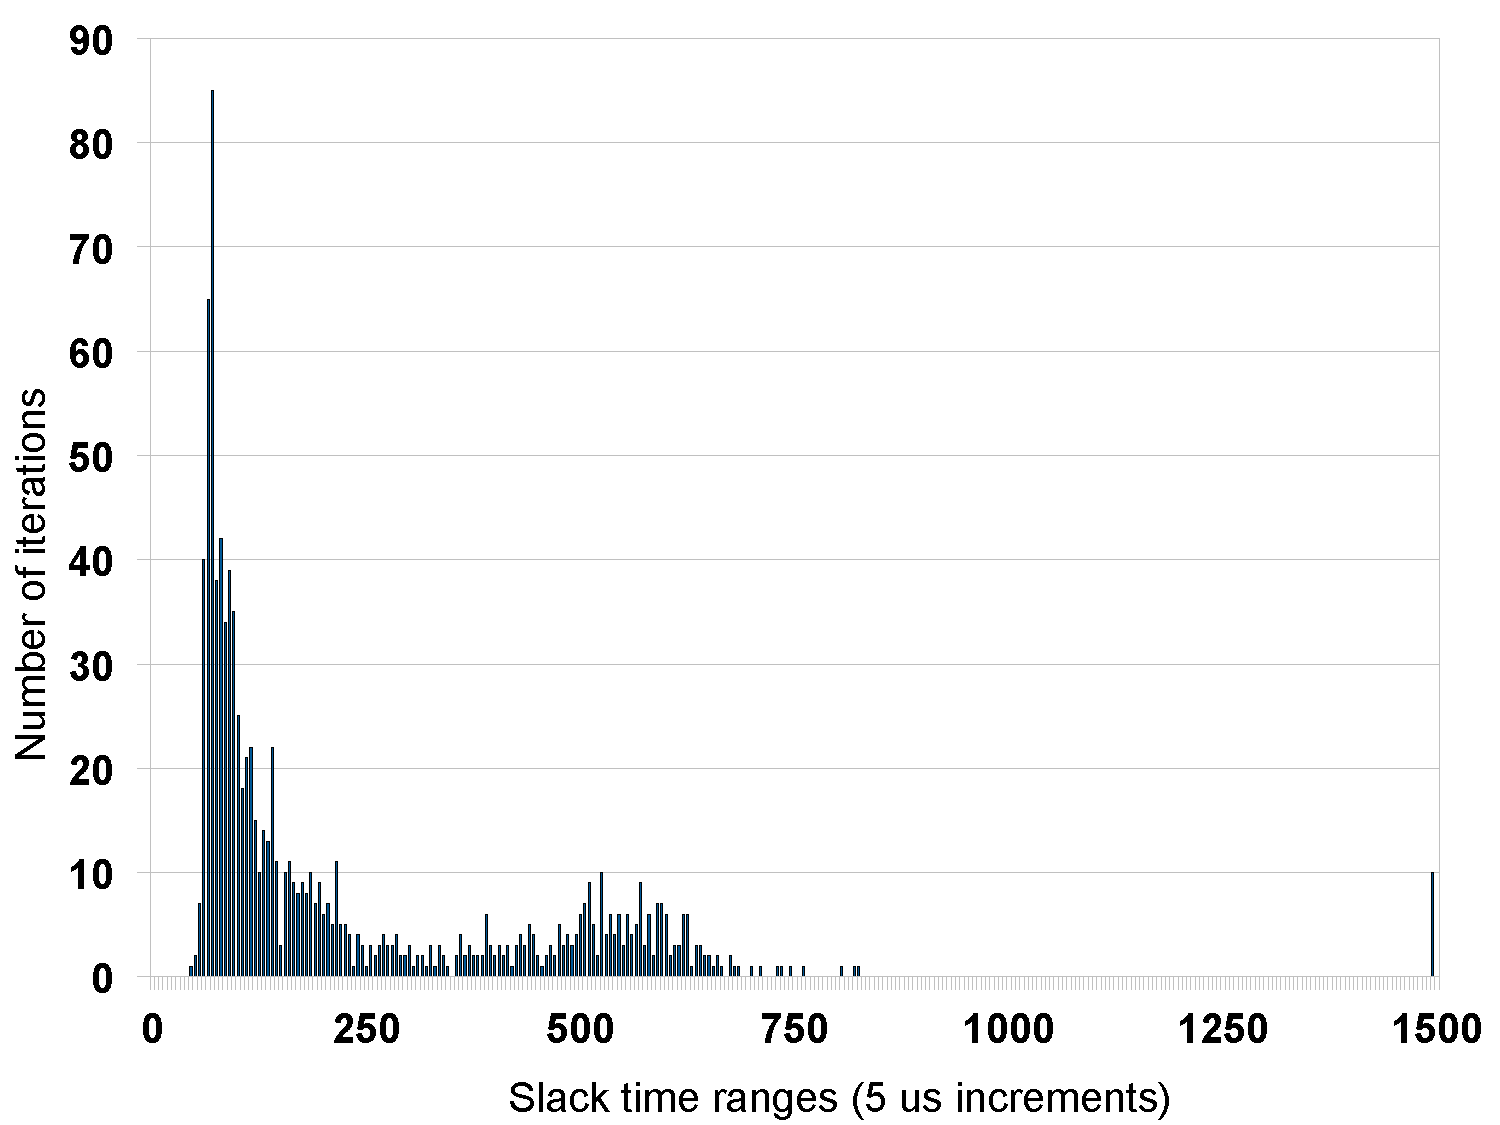
\includegraphics[width=.47\columnwidth]{images/slackVar-allreduce-rank0}
          \caption{  }
        \end{figure}  

        \begin{figure}[htb]
          \centering
          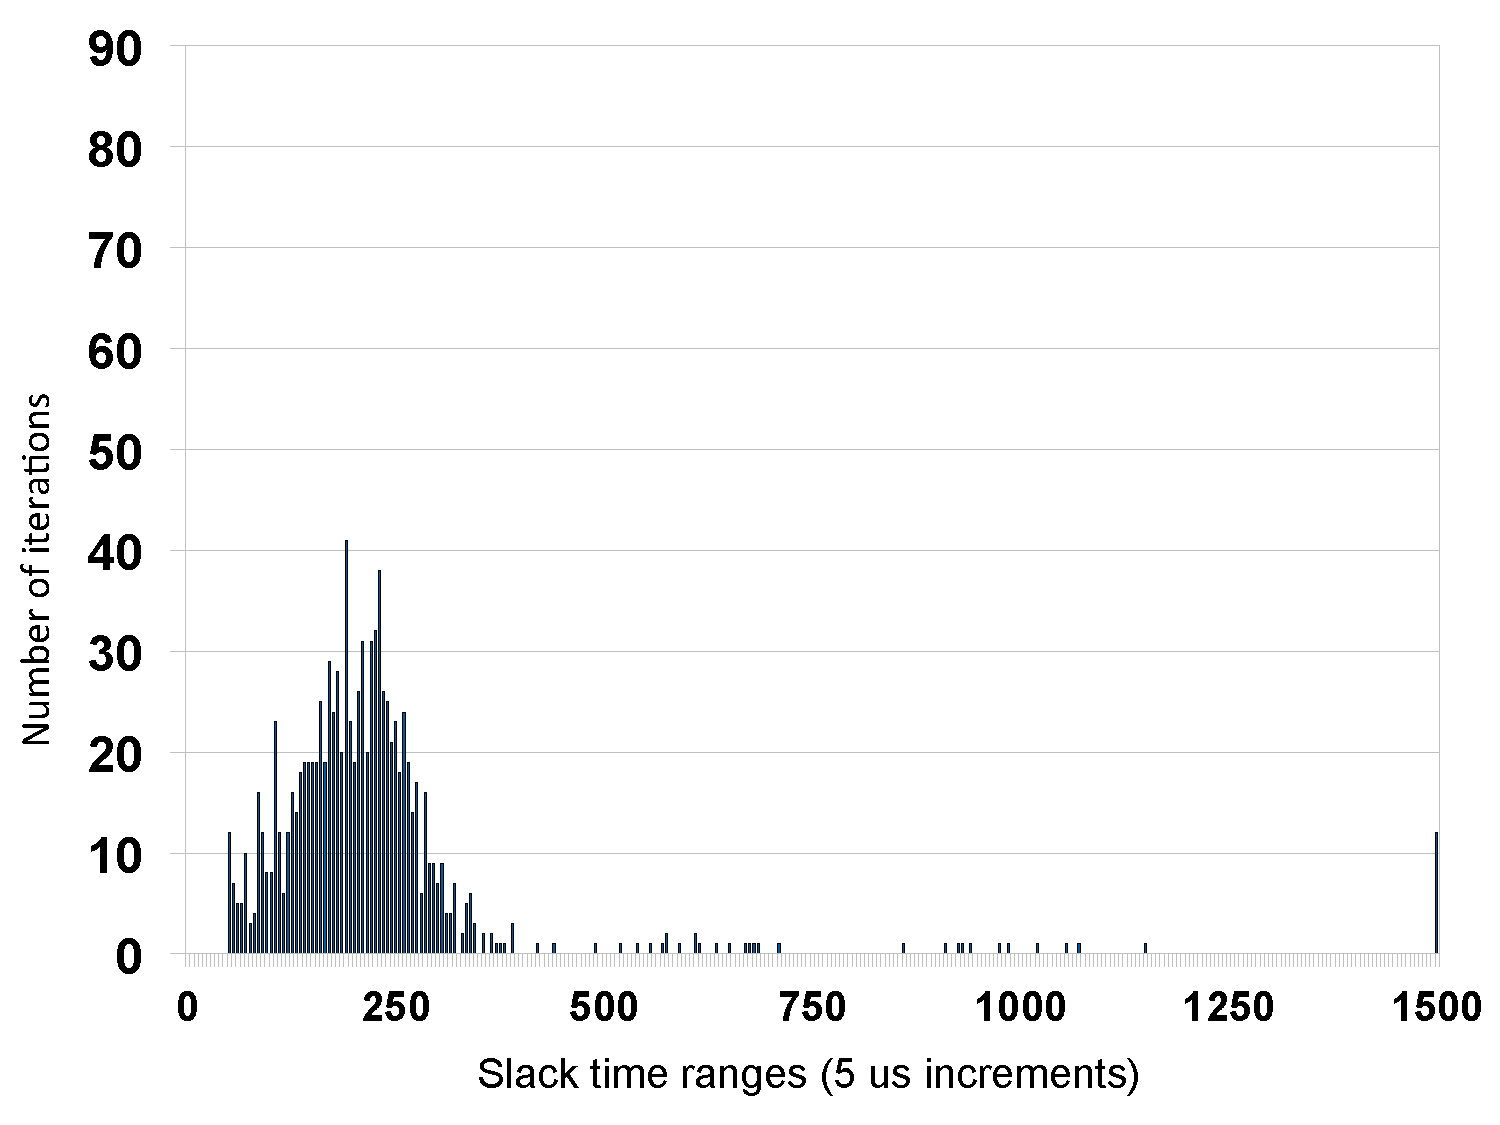
\includegraphics[width=.47\columnwidth]{images/Slack-Histogram-MPI-Allreduce-rank1}
          \caption{       } 
        \end{figure} 
        %\vspace{1ex}
       \begin{columns}[t]
          \begin{column}{0.01\columnwidth}\end{column}
         \begin{column}{0.98\columnwidth}
        \begin{columns}
          \begin{column}{0.47\columnwidth}
          \end{column}\begin{column}{0.40\columnwidth}
            \vspace{1ex}
            \begin{figure}[htb]
            \centering
           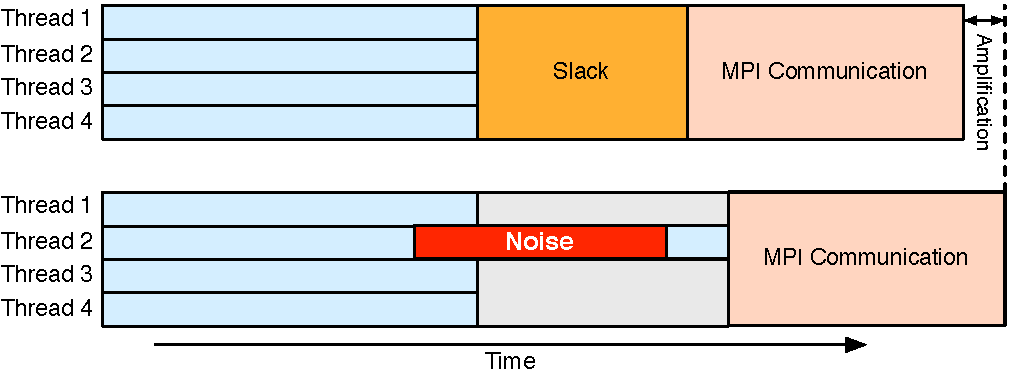
\includegraphics[width=0.8\columnwidth]{images/static-schedule}
            \end{figure}
          \end{column}\begin{column}{0.06\columnwidth}
          \end{column}\begin{column}{0.40\columnwidth}
            \begin{figure}[htb]
            \centering
            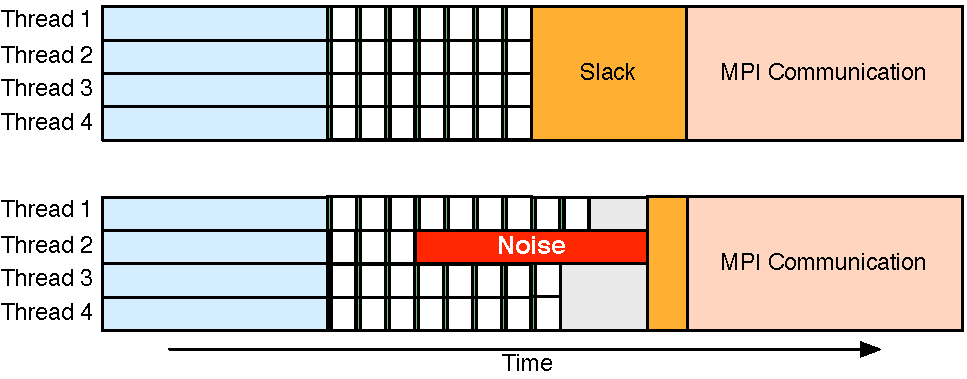
\includegraphics[width=0.8\columnwidth]{images/dynamic-schedule}
           \end{figure}
         \end{column}\begin{column}{0.07\columnwidth}
          \end{column}
        \end{columns}
             \begin{figure}[h]
               \caption{ }
             \end{figure}
           \end{column}\begin{column}{0.01\columnwidth}\end{column}
         \end{columns}
      \end{block}

    \end{column}%2

    %-- Column 3 ---------------------------------------------------
    \begin{column}{0.28\linewidth} 
      %-- Block 3-0
      \begin{block}{}
        \begin{columns}[t]
          \begin{column}{0.01\columnwidth}\end{column}
          \begin{column}{0.98\columnwidth}
 
        \begin{columns}
          \begin{column}{0.07\columnwidth}
          \end{column}\begin{column}{0.07\columnwidth}
            \vspace{1ex}
            \begin{figure}[htb]
            \centering
            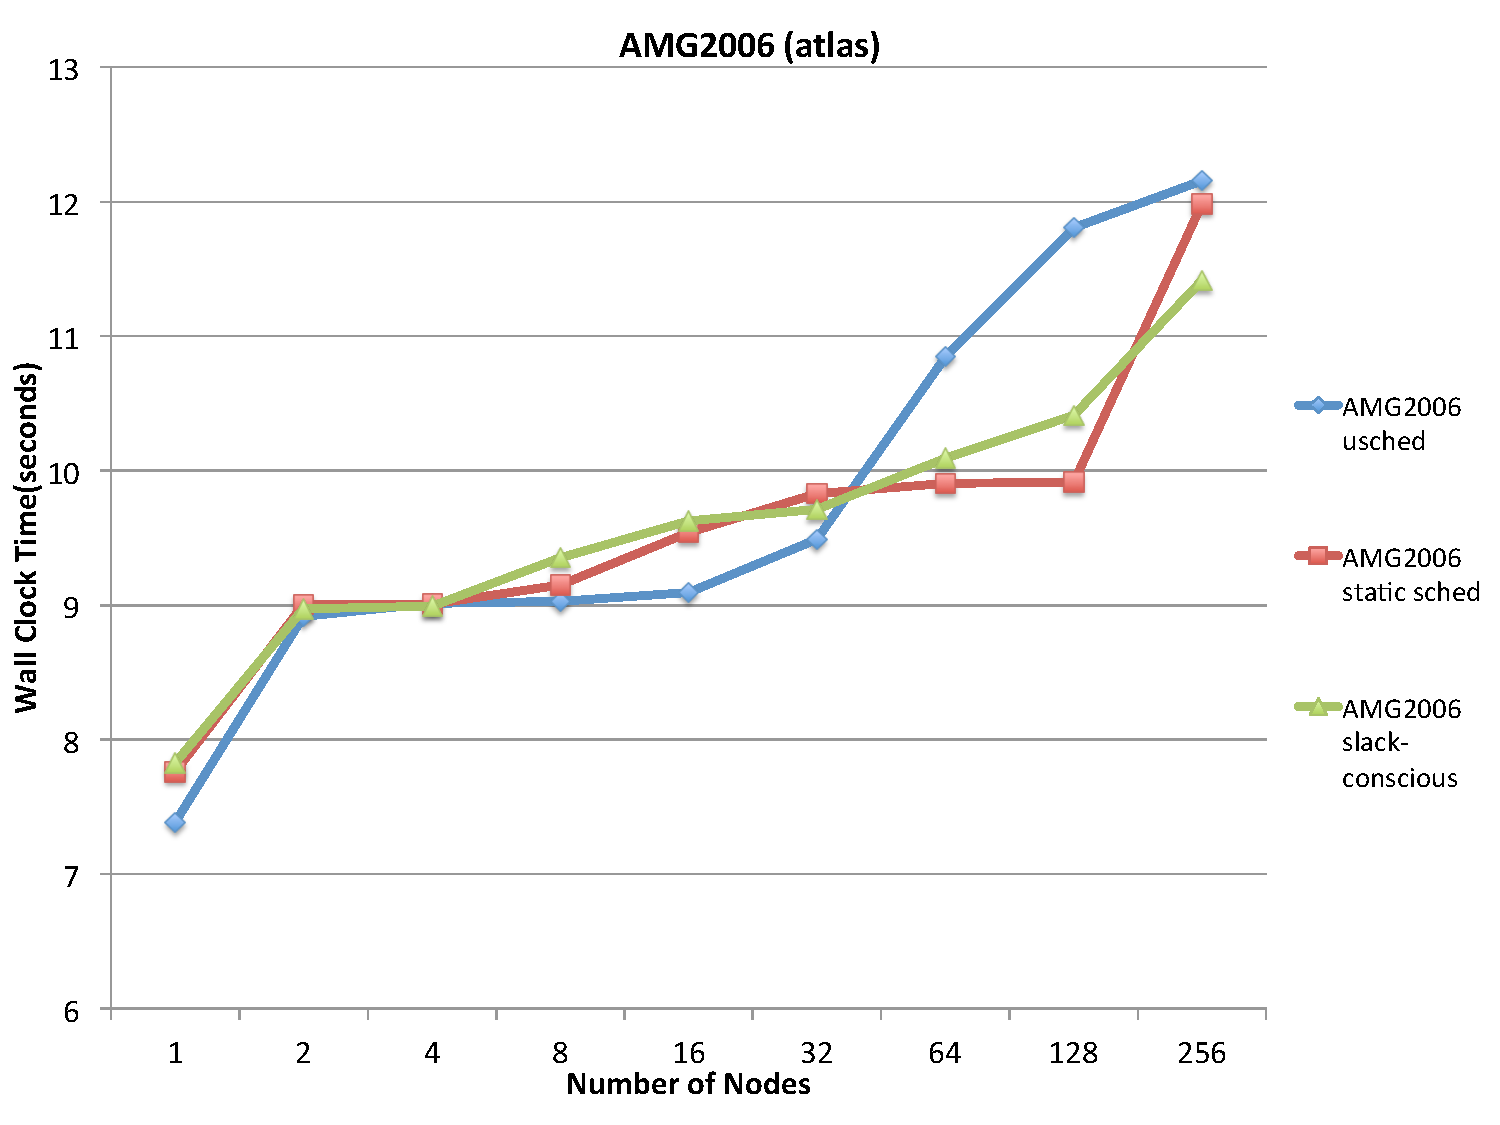
\includegraphics[width=1\columnwidth]{images/AMG-atlas-scaling}
            \end{figure}
          \end{column}\begin{column}{0.07\columnwidth}
            \begin{figure}[htb]
            \centering
            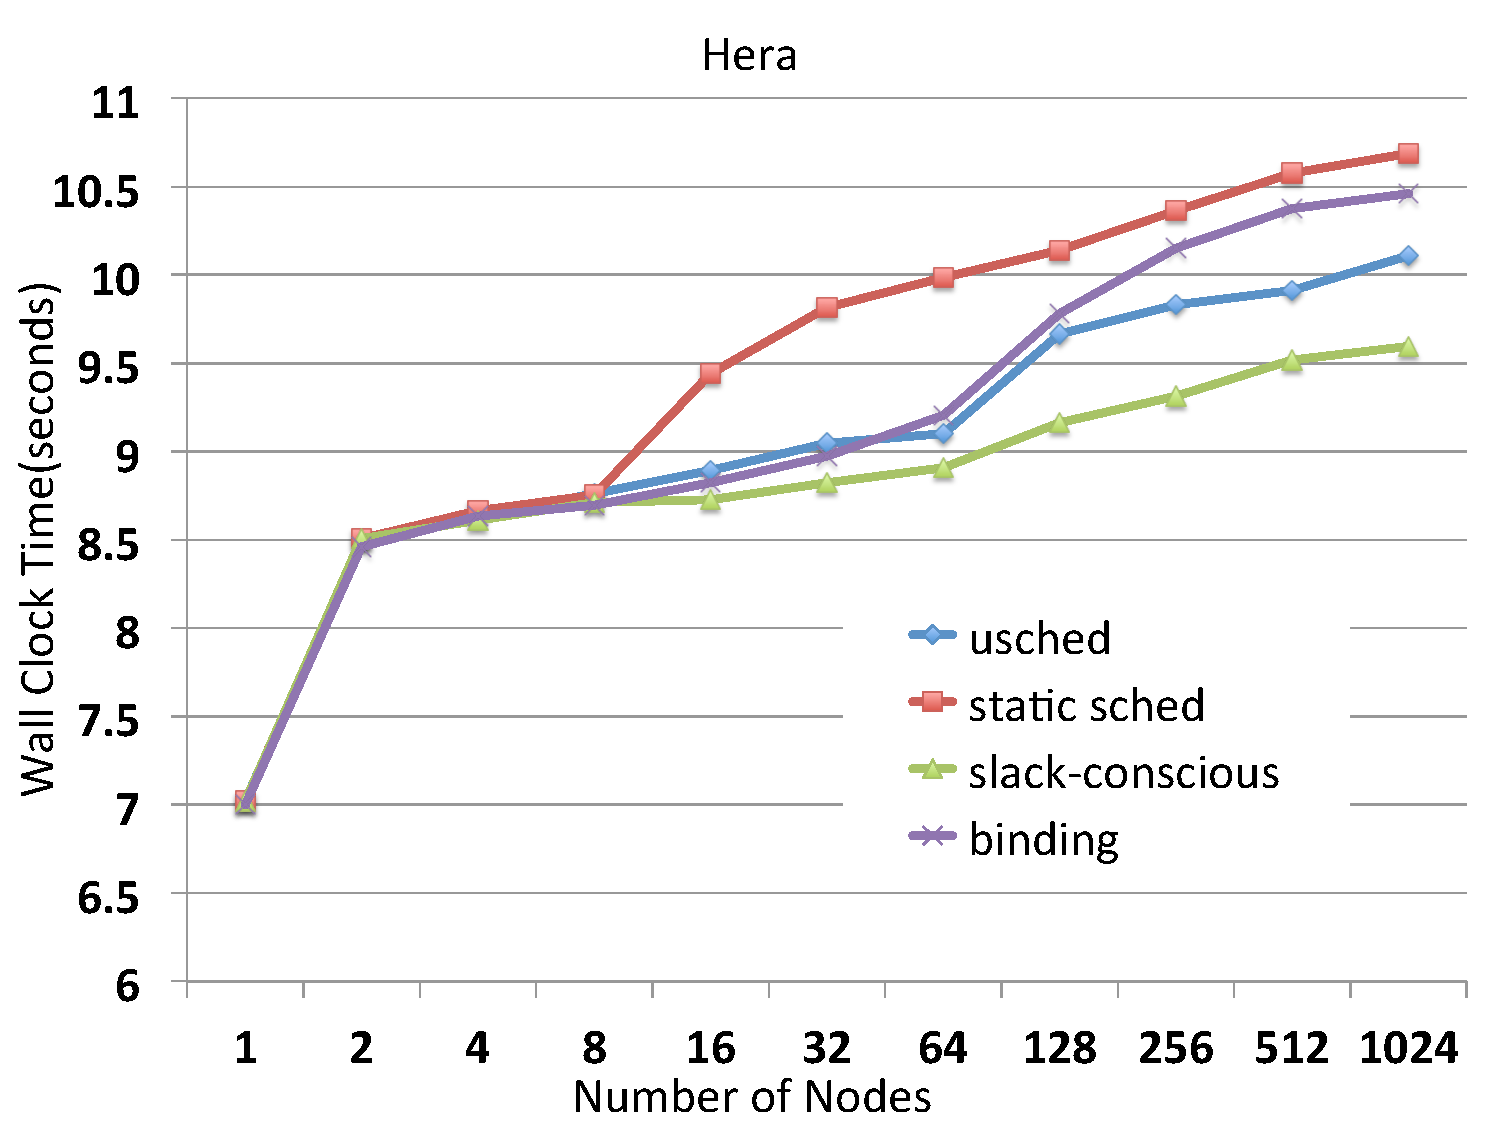
\includegraphics[width=1\columnwidth]{images/AMG-scaling-hera}
            \end{figure}
          \end{column}\begin{column}{0.07\columnwidth}
          \end{column}
        \end{columns}
             \begin{figure}[h]
               \caption{}
             \end{figure}
           \end{column}\begin{column}{0.01\columnwidth}\end{column}
         \end{columns}
      \end{block}
    \vspace{1.5ex} 

      %-- Block 3-1
      \begin{block}{}
        \begin{columns}
          \begin{column}{0.05\columnwidth}\end{column}
          \begin{column}{0.9\columnwidth}  
            \begin{figure}[htb]
              \centering
              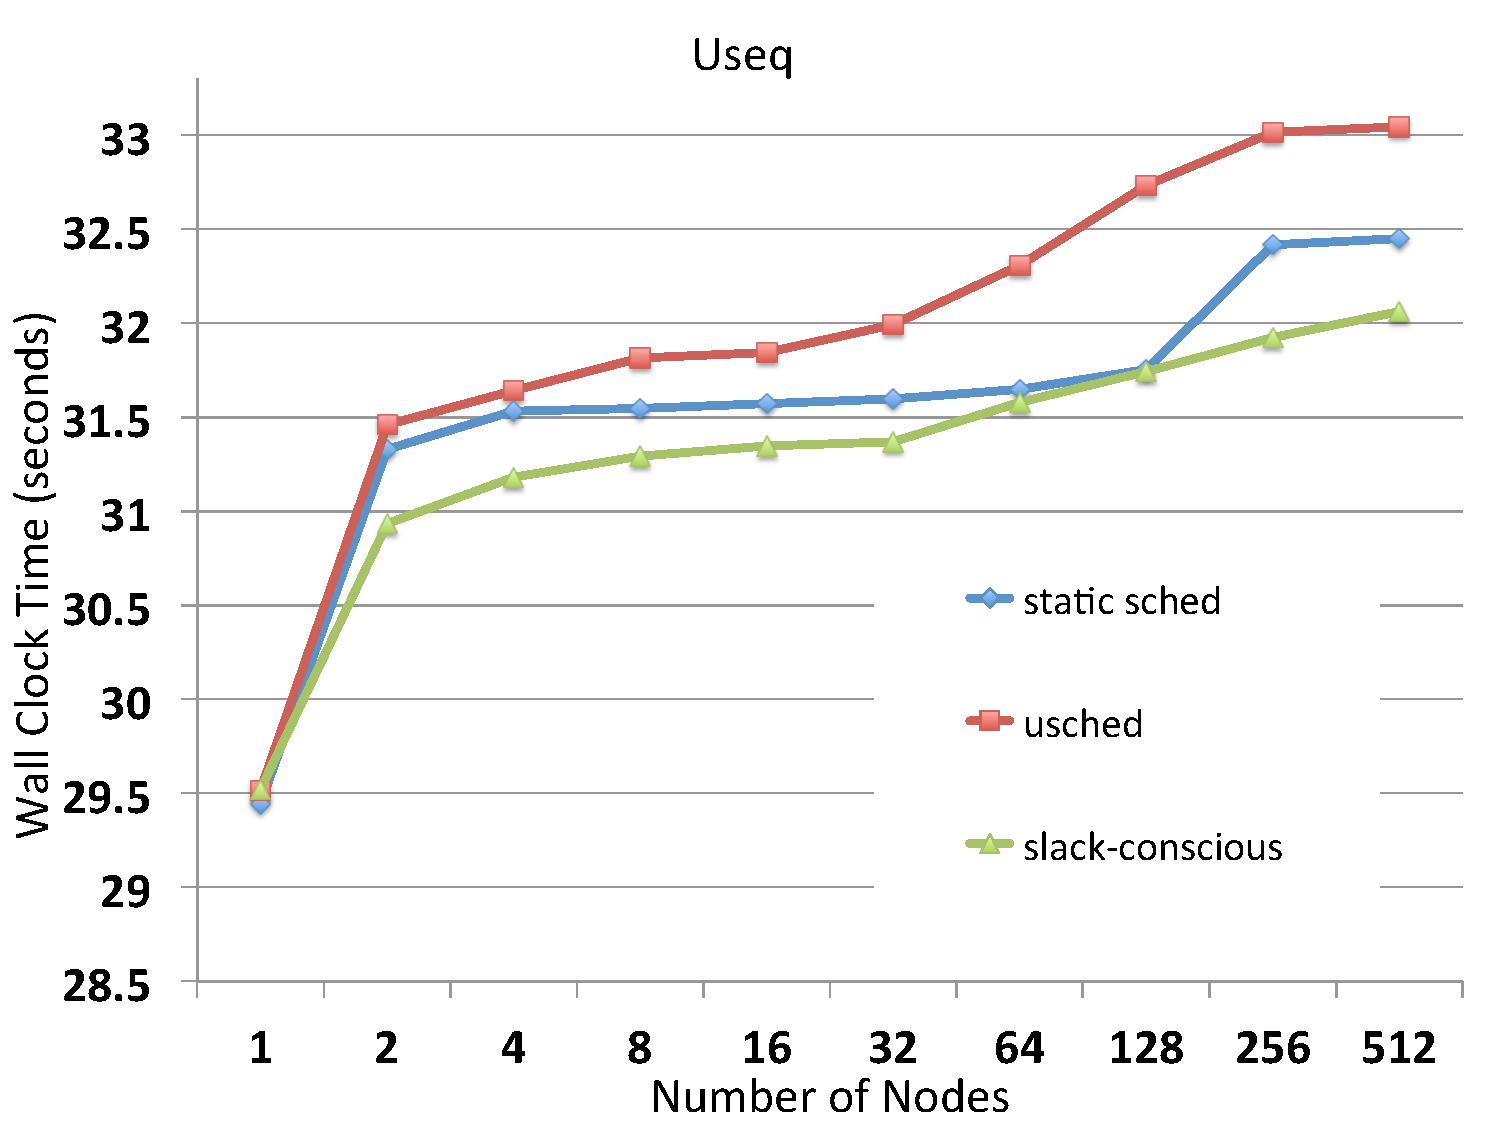
\includegraphics[width=0.44\columnwidth]{images/AMG-scaling-rzuseq}
              \caption{   }
            \end{figure}
          \end{column}
          \begin{column}{0.05\columnwidth}\end{column}
        \end{columns}
      \end{block}

      \vspace{1.5ex}       
      %-- Block 3-3
      \begin{block}{} 
      \end{block}
    \end{column}%3

  \end{columns}
 \end{frame}
\end{document}
